\chapter{Background Knowledge}
\label{Background Knowledge}
\indent \indent This chapter introduces concepts and algorithms that are used in this research.

\section{Genetic Algorithm}
\indent \indent Before discussing about genetic algorithms, we visit its hypernym: evolutionary algorithms. Evolutionary algorithms mimic the biological evolution that living beings use to maintain the existence of their species \cite{GA02}: how each generation's lifetime starts and ends and how optimized it performs its ``tasks," compared to other individuals and its parents \cite{GA03}. In evolutary algorithms, ``organisms'' or a model would naturally survive if it has a stronger gene, for example, when it can perform more optimal problem solving capability \cite{GA01}. The keyword ``gene" here introduces us to the concept of ``genetic algorithms."

Genetic algorithms train individual models in a generation to solve a problem: the outcome being trained models and their respective properties (genes), forming a ``gene pool." Each ``genotype'', consists of a set of genes, is represented by a binary string. Only those with higher fitness value can survive and can reproduce in the next training generation. For each iteration, genes from different qualified individuals can recombine with each other or mutate, just like biological gene crossover or mutation \cite{GA01, GA04}. The generational trainings come into when a stop condition has been met.

A classic pseudocode of genetic algorithms is as follows.

\begin{algorithm}
\caption{A Classic Process of Genetic Algorithms \cite{GA05}}
\label{alg-GA}
	obtain initial population\;
	calculate each individual's quality\;
	\While(\tcp*[f]{produce new generation}){not $completed$}{
		\For(\tcp*[f]{recombination cycle}){$population\:size / 2$}{
			choose two individuals to recombine, prioritizing higher quality candidates\;
			recombine the selected two to produce two offspring\;
			calculate each offspring's quality\;
			append the produced individuals into the new generation/iteration\;
		}
		\If{population count converges}{
		{$completed \gets$ TRUE}
		}
	}
\end{algorithm}

\section{Artificial Neural Networks (ANN)}
\indent\indent Artificial Neural Networks (ANN), or in short neural nets (NN), is an interconnected layers of "neurons" that act as processing elements. Connection strength between neurons, which denotes the processing ability of the network, is represented by "weights" \cite{NN01}. ANN is based on the working of living creatures' nervous systems, especially the brain. As concisely aforementioned, a simple NN consists of layers, neurons, and weights, see Fig. \ref{fig:3ann}. In its simplest form, an NN consists of one input layer and one output layer. An input layer can have one or multiple neurons with different values $x_k$ representing the inputted data to the neural network. A weight $w_k$ connects an input neuron $w_k$ and an output neuron $y$ and acts as a multiplier, i.e. the output neuron $y$ will receive the value $w_k{}x_k$ from this connection. A neuron can be a source of multiple weights to the next layer and also a destination of multiple weights from the previous layer. The value of a output layer neuron in Fig. \ref{fig:3ann} is equal to $y = f(\sum^{n-1}_{i=0}w_i{}x_i-\theta)$, where $f$ is an activation function, e.g. Sigmoid, normalization, etc. and $\theta$ an internal threshold or offset. Lastly, the output layer, after receiving its final value, becomes the output of the NN. An output layer is useful for classification problem: it shows which neurons have a value that lies within a specific classification threshold.

\begin{figure}[h]
    \centering
    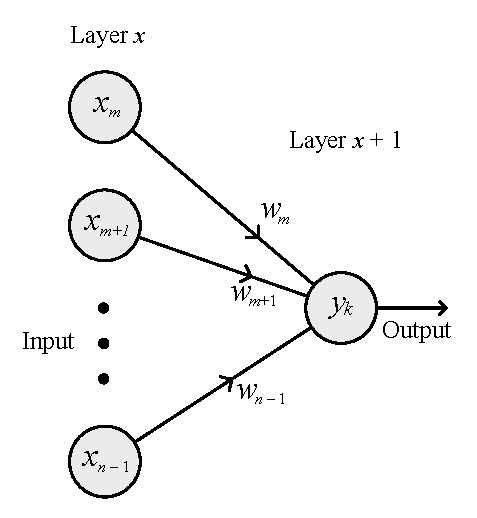
\includegraphics[width=0.35\textwidth]{graphics/3ann.pdf}
    \caption{Structure of an ANN \cite{NN01}}
    \label{fig:3ann}
\end{figure}

The correctness or quality of an ANN can be determined using a loss function, which indicates the disparity between the expected output and the prediction produced by the ANN. Loss function may also be used to adjust other hyperparameters, such as weights \cite{NN02}.

%/parameter, hyperparameter
%/construction
%/loss fn etc
%/prediction
%/tuning/optimization
%/uses

\subsection{Deep Learning}
Deep learning improves ANN in a way that it is multi-layered: each layer processes different levels of features. Deep learning algorithms have intermediary layers between the input and output layers which in a progression extract useful input patterns and pass them to the subsequent layer \cite{NN03}. According to how inputs are presented or obtained, deep learning can be divided into multiple types, most prominently (1) supervised learning, (2) unsupervised learning, (3) reinforcement learning, or (4) combination between any of (1), (2), or (3).

Supervised learning problems has the following characteristics. First, data is presented in the form of $X \mapsto Y$, where $X$ is a representation data labeled with a label $Y$. Next, the learning agent will abstractly learn the relations between $X$ and $Y$ as a knowledge base to predict the label of a new input. Unsupervised learning lacks $Y$ part such that the learning agent needs to infer data classification from the feature distribution of input data. Agents in reinforcement learning learns independently, assisted from rewards and punishments from performing an action in one environment state.

\section{Analytic Trading}
\indent\indent Trading, in this sense, refers to an activity of buying, selling, or holding a commodity, stock, currency, or other derivative assets in their corresponding finacial markets. The ultimate goal of trading is to gain profit from price difference and minimizing transactional cost. Analytic trading optimizes profit-making decisions by predicting price actions based on fundamental analysis plus chart features such as price trend, support and resistance levels, trading volume, trading indicators, price patterns, etc. \cite{AT52}. Fig. \ref{fig:3tv} shows Bitstamp's Bitcoin-USD pair chart taken from TradingView on 5 August 2022, at 9:01 AM UTC. It contains different indicators: Volume (Vol), Moving average with window size equals 28 bars (MA(28)), MACD long/short strategy, and Bollinger Bands with window size 20 and band deviation of 2 sigma (BB(20,2)).

\begin{figure}[h]
    \centering
    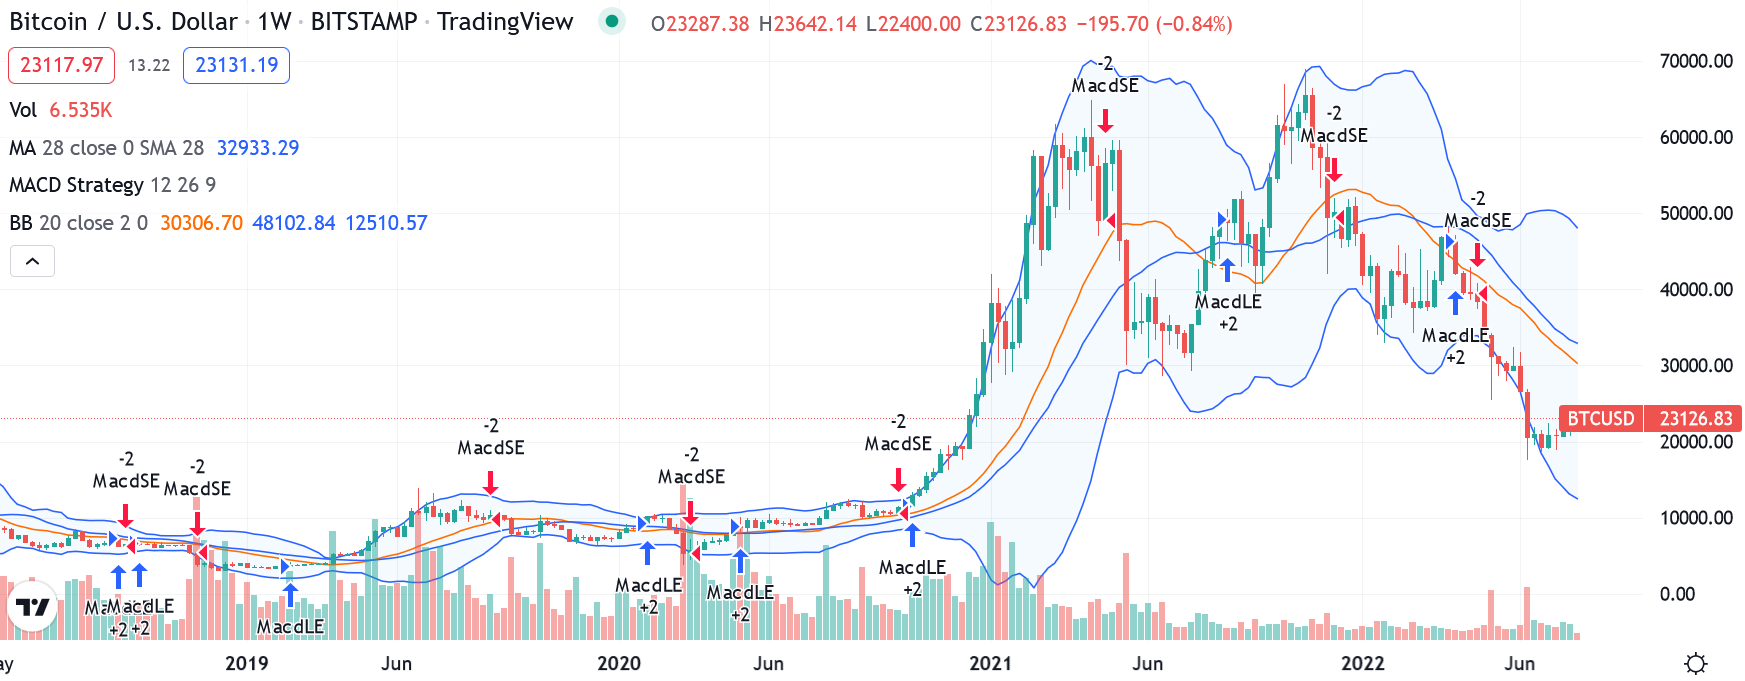
\includegraphics[width=0.96\textwidth]{graphics/3bitcoinindicators.png}
    \caption{An example of trading chart with several indicators \cite{X001}}
    \label{fig:3tv}
\end{figure}

Typically, the input data of a price prediction problem is in a form of a time series data \cite{AT51}. Values from a time window is then calculated and analyzed to obtain various indicators to assist trading decision. More recent approaches automate trading decisions in a form of algorithmic (algo) trading, which can generate decisions in (near-)real time. Sometimes, algo trading is empowered by artificial intelligence and ANN to improve the prediction performance as well \cite{AT49}.

Many fund managers nowadays have shifted their interest to trade cryptocurrencies due to their profit-inducing volatility \cite{AT72} and rapid development \cite{AT71}. Bitcoin, being the first invented and the most mature cryptocurrency, has become the cryptocurrency standard in various researches and studies \cite{AT72}.

There are three basic actions in spot trading: \texttt{Buy}($x$) or \texttt{Long}, \texttt{Sell}($x$) or \texttt{Short}, and \texttt{Hold}. \texttt{Buy}($x$) tells the trading bot to buy $x$ units of asset at the specified time, \texttt{Sell}($x$) works similarly but for selling, and \texttt{Hold} is to neither buy nor sell the asset at the specified time point. Decision to choose one of the three depends on indicators, or in ANN-enhanced decision, the output of the ANN.

This research uses two popular indicators: exponential moving average (EMA) and Moving Average Convergence/Divergence (MACD), a derivative of EMA. $EMA$($x$) is defined as
\[
	EMA(x) = p \cdot k + EMA_p \cdot (1 - k),
\] where $n = \frac{2}{x+1}$, $x$ is the number of time frames considered in the EMA, $p$ is the asset price at the current timeframe, and $EMA_p$ is the value of EMA of the previous day \cite{AT22}. Since the function is recursive, the base case of the formula, for the first datapoint, is \cite{AT23}
\[
	EMA_0(x) = \frac{\sum_{i=0}^{t - 1} p_i(1-\alpha)^i}{\sum_{i=0}^{t-1}(1-\alpha)^{i}},
\] where $\alpha$ is the discounting factor of past values, typically is 0.18.

MACD, on the other hand, uses EMA in its calculation, and is defined as: $MACD(f, s)$ = $EMA(f) - EMA(s)$. $f$ stands for ``fast" moving average, typically is fixed at 12. $s$ is ``slow" moving average, typically is equal to 26. On top of that, $EMA(l)$ of $MACD$ is called the ``signal line", equals to $EMA(l) - MACD(f, s)$ \cite{AT23}. Signal line (hereafter notated by $\sigma$) is useful to trigger buy and sell signals. When $MACD - \sigma$ turns from negative to positive, a buy signal is issued; when it turns from positive to negative, a sell signal is issued. Otherwise, no trade is done.

\subsection{Deep Learning for Trading}
\label{sec:dl}
Long-Short Term Memory (LSTM), a subset of Recurrent Neural Network (RNN), is a popular supervised deep learning algorithm for trading bots since its nature fits with predicting future values from past data. This class of RNN uses either sigmoid or hyperbolic tangent (tanh) activation function and SoftMax. Back propagation in RNN, when seeing a non-optimal result, may redirect the outputs of the network to the hidden, intermediary layer, in a hope to improve the prediction result \cite{AT20}.

LSTM improved long-term forecasting by adding more memory into RNN. Each LSTM `cell' (Fig. \ref{fig:3lstm} \cite{NN05}) has two states: hidden state ($h$, to process input and output and short-term memory) and cell state ($c$, for data flow and long-term memory). There are several steps in building an LSTM network \cite{NN04}. First, forgetting unused information from previous step ($h_{t_1}$) and input $X_t$ using a sigmoid function ($\sigma$) through the forget gate ($f_t$, a vector whose values are between 0 and 1). The next stage is remembering new information from $X_t$ through the memory gate ($i_t$ to accept or discard new information multiplied by $\tilde{C}_t$ to give an importance level to the input). Finally, the output of the cell $h_t$ is obtained by multiplying $\sigma(h_{t_1})$ and $c_t$.

\begin{figure}[h]
    \centering
    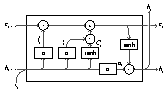
\includegraphics[width=0.48\textwidth]{graphics/3lstm.pdf}
    \caption{An LSTM cell}
    \label{fig:3lstm}
\end{figure}

LSTM, in this regard, however, is used mostly for forecasting stock prices. Trading decisions are generated using another deep learning algorithm called Convolutional Neural Network (CNN). CNN, usually used for feature extraction in multidimensional spaces like images, learns stock movement patterns (trend, trajectory) and thus can decide when to buy or sell an asset \cite{AT21}. Not many works indicate the ROI, but prediction accuracy. Yet, Chakole and Kurhekar's work \cite{AT21} show that a plain CNN would return a lower ROI than other methods, including the buy-and-hold method.

\section{Markov Decision Process (MDP)}
\indent\indent Markov Decision Process is central to the main concept of this research Reinforcement Learning (RL). MDP mimics the working of decisions in human life, focuses on choosing the better impact from decisions. MDP can be modeled after a finite state machine like in Fig. \ref{fig:3mdp}. An agent can choose to go from a state to another state (or back to its current state) via an action and receive a reward for each state propagation. In a more general definition, an agent can act upon the environment to move to another state and receive a reward as a consequence \cite{ML01}.

\begin{figure}[h]
    \centering
    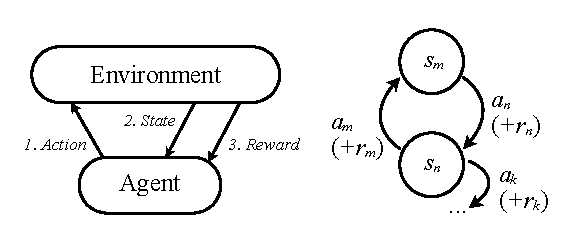
\includegraphics[width=0.66\textwidth]{graphics/3mdp.pdf}
    \caption{Markov Decision Process in two views.}
    \label{fig:3mdp}
\end{figure}

The formulation of MDP is as follows \cite{ML01}:

\[
r_t(s,a)=\sum_{s'\in{}S}r_t(s,a,s')p_t(s'|s,a),
\]

where $r$ denotes reward, $t$ is the current propagation instance, $r_t(x)$ is the reward of performing a propagation $x$, $s$ is the current state, $a$ indicates the action taken, $s'$ is the next state after performing $a$ on $s$, and $p(x)$ is the probability of propagation with condition $x$ happening.

According to Feinberg and Schwartz \cite{BK01}, there are two kinds of impacts: (1) cost minimization and profit maximalization and (2) impacts on future states after the decision. MDP looks for a decision that is profitable in long-term period by choosing optimal policies. MDP is shown to be useful in various implementations. In finance and investment, \cite{BK03} uses MDP to decide when to sell or hold a financial asset to get faster gain. Saario \cite{BK04} tries to solve a house-selling problem, that is, someone must decide to sell a house given an arbitrary offer or decline the offer and wait longer for a better offer. An MDP-like dynamic programming (DP) solution is used to maximize the accepted offer value.

\subsection{Bellman Equation and Optimality}
% Bellman, Bellman optimality
Bellman equation plays an important role in dynamic programming: it expects the total reward from the present state $s$ to the end of the propagation horizon in an MDP. The equation \cite{ML01} is as follows:

\[
v^{\pi}_t(s) = \max_{{a\in{}A(s)}}\left\{r_t(s,a)+\sum_{s'\in{}S}\gamma^t p(s'|s,a)v_{t+1}(s')\right\},
\]

where $v^{\pi}_t(s)$ is the expected present and future total rewards from the current state $s$. A discounting factor $\gamma^t$, $0 < \gamma < 1$ is sometimes added to diminish the effect of far-future rewards and to put priority to near-future rewards.

The best and most optimal possible $v^{\pi}_t(s_0)$ is denoted by $\max_{\pi}v^{\pi}(s) = v*(s)$. Bellman's Optimality Theorem states that \cite{BK05} $v^*(s)$ must satisfy the Bellman Optimality Equation
\[
	v^*(s)=\max_{a}\left\{r(s,a)+\gamma{}\sum_{s'}p(s'|s,a)v^*(s')\right\}
\] for all $s$.

\section{Reinforcement Learning (RL)}
\indent\indent Reinforcement Learning (RL), a branch of deep learning, is analogous to how living things learn to perceive and to interact with their environment: by doing something experimentally then receiving a reward or a punishment as a consequence \cite{RL01}. Like so, RL iteratively learns causes and effects under little supervision to reach the goal of obtaining as much reward as possible, in a computational way.

Based on finite MDP, RL can be illustrated using Fig. //ADD FIGURE HERE// \cite{RL01}. Five elements of RL are :
\begin{enumerate}
	\item Agent: the entity which learns about the environment by taking actions and receiving rewards,
	\item Environment: every entity other than the agent whom the agent interacts with,
	\item State $S_t$: the current state or constellation of the environment,
	\item Action $A_t$: a set of tasks or actions that the agent can take at the current state to change the state of the environment, and
	\item Reward $R_t$: the consequence that the agent receives upon completing an action.
\end{enumerate}

\subsection{Policy in RL}
The output of RL is a policy $\pi_t$ for each time step, that is, $\pi_t(a|s)$, a probability of choosing an action $A_t = a$ given the current state $S_t = s$. The ultimate goal is to produce a set of policies $\pi_t$ for every $A_t$, $S_t$ which maximizes $R_t$ in the long run. In an equation \cite{QL03},

\[\pi^* := \argmax_x \mathbb{E} \left[ \sum_{k=0}^{\infty} \gamma^k{}r_k \middle| \pi \right],\]

where $\pi^*$ is a deterministic optimal policy, $\mathbb{E}[\cdot|\pi]$ is expectation based on policy $\pi$, $\gamma$ is discount factor, which determines agent's consideration of possible future actions. $\pi$ itself describes the policy under a state-action trajectory $s_0, a_0, s_1, a_1, ..., a_{k-1}, s_k$.

\subsection{RL Taxonomy}
The following list adopted from \cite{RL07} shows the taxonomy of RL algorithms. Some of the subbranches and algorithms will be discussed in the subsequent paragraphs.

\begin{enumerate}
	\item Model-Based RL
	\begin{enumerate}
		\item Model given, e.g., \texttt{MCTS} (Monte Carlo tree search)
		\item Model learned, e.g., \texttt{I2A} (Imagination-Augmented Agents), World Model
	\end{enumerate}
	
	\item Model-Free RL
	\begin{enumerate}
		\item Value-Based: focus on state-action value
		\begin{enumerate}
			\item On-Policy: policy determines learning
			\begin{itemize}
				\item \texttt{Sarsa}
			\end{itemize}
			\item Off-Policy: learning is done randomly
			\begin{itemize}
				\item \texttt{Q-Learning}
				\item \texttt{DQN} (Deep Q-Network), 
				further classified into \texttt{C51},
				\texttt{Dueling DQN}, \texttt{Double DQN}, \texttt{QT-Opt},
				and \texttt{DDPG} (Deep Deterministic Policy Gradient).
			\end{itemize}
		\end{enumerate}
		\item Policy-Based: focus on overall policy value
		\begin{enumerate}
			\item Gradient-free
			\begin{itemize}
				\item Cross-Entropy Method: \texttt{QT-Opt} (intertwined with \texttt{DQN})
				\item Evolution Strategy: \texttt{SAMUEL}
			\end{itemize}
			\item Gradient-based
			\begin{itemize}
				\item \texttt{Policy Gradient}
				\item \texttt{TRPO/PPO} (Trust Region Policy Optimization/Proximal Policy Optimization)
				\item \texttt{ACKTR} (Actor Critic using Kronecker-Factored Trust Region)
				\item Actor-Critic
				\begin{itemize}
					\item \texttt{A2C} (Advantage Actor Critic)
					\item \texttt{A3C} (Asynchronous Advantage Actor Critic)
					\item \texttt{DDPG} (Deep Deterministic Policy Gradient), combined with \texttt{DQN}: \texttt{TD3} (Twin Delayed DDPG), \texttt{SAC} (Soft Actor Critic)
				\end{itemize}
			\end{itemize}						
		\end{enumerate}
	\end{enumerate}
\end{enumerate}

\subsubsection{Model-based and Model-free Reinforcement Learning}

A model in RL refers to any data or knowledge that contains the state-action-reward prediction table for an agent to plan and follow. Model-based RL uses a model, learned or known, and approximates a policy function from learning \cite{RL04}. Model-free RL, on the other hand, calculates the environment spontaneously using trial-and-error, while retaining no transition probability distribution arrays, hence learning how to act solely based on rewards \cite{RL05}. Model-free algorithms are viewed to be labor-intensive but can adapt to new environment fast, while model-based algorithms are more lightweight but produce less optimal policies, hence are more suitable for deterministic use cases.

\subsubsection{Actor-Critic Method}
Konda and Tsitsiklis \cite{RL06} observe that most RL algorithms are either actor-only or critic-only. Actor-only methods focus on parametrization of policies and parameter improvisation without learning process. An example of actor-only methods is REINFORCE. Critic-only methods use solely value approximation in learning to comply with the Bellman equation, but produce less optimal policy. An example of critic-only methods is Q-learning.

Thus, the actor-critic method is derived to fuse the advantages of actor-only and critic-only algorithms. Actor-critic mathods typically use two separate neural networks: a neural network for actor and a neural network for critic \cite{RL101}. The critic part approximates and simulates learning to improve the actor segment's policy parameters.

\subsubsection{Policy Gradient}
% grad descent explained in short only
Actor-critic algorithms often use the policy gradient theorem \cite{RL07}. However, Sutton et al. \cite{RL27} claim that sole function approximation is not effective enough in realizing a policy convergence. One effort is to parametrize the policy instead of computing the policy from parametrized action-value functions. This way, one can track and plan the gradient descent of the overall policy parameter. Say that the policy parameter is denoted by $\theta$, the gradient $\Delta\theta = \alpha\hat{\nabla}_\theta{}J(\theta)$ can be adjusted by setting $\alpha$: step size and $J(\theta)$: RL performance of the policy that follows the parameter $\theta$, either calculated by total reward or reward per step.

\paragraph{Gradient Descent}
Gradient descent itself is a method that iteratively minimize a function value. Imagine a function $y = f(x_1, x_2, ..., x_n)$. Gradient descent starts with choosing a random or predefined parameter vector $x_1, x_2, ..., x_n$ as the initial position. Obtain the gradient vector by observing the change of $y$ when each of $x_1, x_2, ..., x_n$ is changed by a little. Next, adjust some $x$ using a predefined step to get $y$ with smaller value and repeat until a local minima for $y$ is found. This process can be illustrated by Fig. \ref{fig:3gdes}.

\begin{figure}[h]
    \centering
    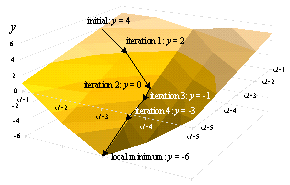
\includegraphics[width=0.66\textwidth]{graphics/3gdes.pdf}
    \caption{Gradient descent}
    \label{fig:3gdes}
\end{figure}

\subsubsection{Q-learning}
\label{qlearning-dqn}
Q-learning is a model-free RL algorithm which explores the maximum reward of all possible state-action propagations, updated for every propagation. The Q-function $Q(s,a)$ is defined as $r(s,a)+\gamma{}v^*(\delta(s,a)) = r(s,a) + \gamma \max_{a'} Q(\delta(s,a),a')$, where $\delta$ is a state transition function. Therefore, in Q-learning notation, $\pi^*(s) = \argmax_{\pi} Q(s,a)$. The maximum current rewards of state-action pairs are recorded in an $n-$dimensional array, and for each iteration, Q-learning will choose the action with the highest reward, based on the current state. The algorithm is as follows \cite{RL01}:

\begin{algorithm}
\caption{Q-learning Algorithm}
\label{alg-QL}
	$Q(s,a), \forall s \in S, a \in A(s) \gets$ an arbitrary value\;
	$Q(terminal\:state, \cdot) = 0$\;
	\While{$S$ is not terminal state}{
		$S gets$ initial value\;
		\For{each propagation}{
			Based on $\pi$ constructed in $Q$, select possible $A$ for the current $S$\;
			Perform $A$, get $R$ and $S'$\;
			$Q(S,A) \gets Q(S,A) + \alpha[R + \gamma \max_{a}Q(S',a)-Q(S,A)]$
			$S\gets S'$
		}
	}
\end{algorithm}

\paragraph{Q-learning with Deep Learning}
However, in a system with huge dimensions of $A$ and $S$, calculating $Q$ value for all $S,A$ pairs consumes heavy resources which is unsustainable and inefficient. Mnih et al. \cite{RL03} combine Q-learning with Deep Learning, called a deep Q-network (DQN), to convert high-dimensionality input into a quantized, pattern-matched inputs with lower dimensionality. The work gives an example scenario: an RL agent needs to observe a video game with 84 $\times$ 84 $\times$ 4 consecutive images $\times$ 256 grayscale levels and to act upon the state by ``clicking" on one of many controller buttons. With a plain array-based Q-learning, each state change require the system to recursively calculate $256^{84 \times 84 \times 4} \times 18 \approx 10^{69971}$ Q values, assuming that there are at most 18 different actions that the agent can take. That value exceeds the number of atoms in the universe, which is $\approx 10^{82}$. With DQN, state-action-reward mappings are approximated using convolutional neural network on-the-go and per-request. This way, determining action would not require storing or generating much, and sometimes unnecessary, prior knowledge.

\subsection{This Research's RL Algorithms in A Nutshell}
Alongside with DQN which is introduced in Section \ref{qlearning-dqn}, four RL algorithms are used: Asynchronous Advantage Actor Critic (A3C), Advantage Actor Critic (A2C), Soft Actor-Critic (SAC), and Proximal Policy Optimization (PPO).

\subsubsection{Asynchronous Advantage Actor Critic (A3C) and Advantage Actor Critic (A2C)}
A3C came from a research by Mnih et al. \cite{RL103} that proposes an asynchronous deep RL framework which adds asynchronous, parallel actor-learners over Sarsa, one-step Q-learning, n-step Q-learning, and A2C. The framework is designed such that multiple RL actor-learners are run in different CPU threads, updating a centralized parameter server. The work finds that parallel workers expand the exploration horizon, hence maximizes knowledge procurement and thus learning speed. Among the asynchronized versions of the four base algorithms, asynchronous A2C (thus called A3C) is the fastest agent that reaches the higher score when tested on Atari 2600 games.

A2C, derived in the same work, is a version of A3C with only one agent. In short, A2C is an improvement of vanilla actor-critic method with an addition of \textit{advantage} value: how advantageous it is to take an action $a_t$ compared to the average of all possible actions at the state $s_t$ \cite{RL103W}.

\subsubsection{Proximal Policy Optimization (PPO)}
OpenAI's Schulman et al. \cite{RL102} derived a family of algorithms called the Proximal Policy Optimization (PPO) algorithms, a subset of policy-based RL. PPO improves Trust Region Policy Optimization (TRPO) in terms of implementation, sample complexity, and execution time. For one eposide of policy update, PPO goes through multiple or batched small episodes of stochastic gradient policy ascent. Moreover, PPO focuses on the area of policy gradient change with high probability, to increase policy faster and more efficiently. Tested using benchmark RL tasks (\texttt{Hopper-v1}, \texttt{Walker2d-v1}, \texttt{HalfCheetah-v1}, etc.), PPO is claimed and shown to perform better than A2C, CEM, TRPO, A2C with Trust Region, and vanilla Policy Gradient method.

\subsubsection{Soft Actor-Critic (SAC)}
An example actor-critic algorithm that combines policy-based and value-based RL is Soft Actor-Critic (SAC) \cite{RL100}. SAC optimizes policy function using an off-policy way by mimicking Q-Learning's approach to accomplish a task: by acting balancedly random (maximizing entropy) yet also enhancing expected reward. The original work \cite{RL100} indicates that SAC performs better on benchmark RL tasks (\texttt{Hopper-v1}, \texttt{Walker2d-v1}, \texttt{Ant-v1}, etc.) compared to prior works such as TD3, DDPG, PPO, and Soft Q-Learning (SQL).